\subsubsection*{15.}
Pour afficher la taille de la table SUBSCRIBE en KO , on va selectionner la table
USER\_SEGMENTS depuis DBAIOT , affichant l'attribut BYTES qui donne la taille du segment
en byte(octet) en va le diviser sur \(2^{10}\)(1024) pour converitre au KO et en filtre avec
where segment\_name='SUBSCRIBE' pour just avoir la taille de la table SUBSCRIBE

\lstinputlisting[style=sqlstyle]{SQL/Partie5/size.sql}

\begin{center}
    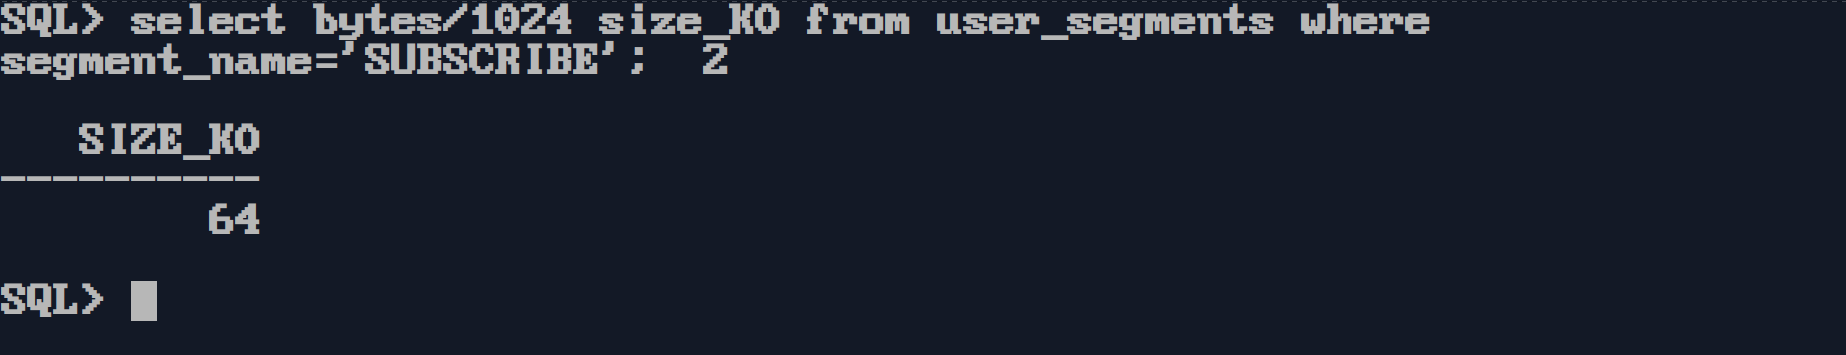
\includegraphics[width=\textwidth]{ScreenShot/Partie5/size.png}
\end{center}


